\chapter{Proposta}

A seguir será detalhado cada ponto proposto neste trabalho em tópicos mais específicos.

\section{O Framework}

A proposta deste trabalho é desenvolver um framework que auxilie no desenvolvimento de redes sociais. Este framework deve oferecer recursos gerais como toda a lógica de usuários e relacionamentos e recursos de rotas e agendas. O recurso de rotas deve ser capaz de fazer um mapeamento de trajetos de interesse de um determinado usuário e auxiliar este a fazer comparações com rotas de outros usuários. A agenda deve oferecer recursos de controle de ocupações no decorrer de dias e horários e auxiliar um usuário a encontrar dias e/ou horários comuns entre um grupo de usuários qualquer.

\subsection{Relacionamento de Usuários}

O relacionamento em redes sociais dá-se por meio de iterações entre os usuários, estas iterações variam de acordo com a rede em que o usuário está inserido. Alguém pode apenas seguir outras pessoas e acompanhar suas postagens, este é um relacionamento unidirecional, pois não é nessário que uma pessoa seguida acompanhe também postagens de seus seguidores. Existe também outro tipo de relacionamento onde é necessário que as duas pessoas estejam diretamente ligadas entre si, o que o torna necessariamente bidirecional, neste tipo pode-se considerar relacionamentos entre conhecidos, amigos, namorados, familiares, entre outros.

Na montagem da estrutura de relacionamentos entre os usuários para redes sociais é nessário fazer uso de grafos onde os usuários serão representados como os vértices e os relacionamentos como as arestas. No caso dos relacionamentos unidirecionais apenas uma aresta é criada. Esta aresta faz uma ligação a partir do vértice do usuário seguidor para o vértice do usuário que este deseja seguir, como pode ser observado na figura \ref{segue}. No caso dos relacionamentos bidirecionais a ligação deverá ser feita usando-se duas arestas paralelas. É necessário que para ambos os usuários exista uma possibilidade de se chegar ao outro, portanto, deve existir uma aresta que ligue um usuário ``A'' a um usuário ``B'' e uma aresta que ligue o usuário ``B'' ao usuário ``A'', vide a figura \ref{amigo}.

\begin{figure}[!h]
	\centering
	\includegraphics[scale=0.45]{figuras/capitulo5/segue.eps}
	\caption{Exemplo de aresta de seguir usuário}
	\label{segue}
\end{figure}

\begin{figure}[!h]
	\centering
	\includegraphics[scale=0.45]{figuras/capitulo5/amigo.eps}
	\caption{Exemplo de arestas pararelas de amizade}
	\label{amigo}
\end{figure}

Cada aresta deverá possuir uma ou mais descrições que detalham qual o relacionamento entre os usuários. Isso fica mais claro ao se falar de relacionamentos bidirecionais, onde pode existir entre duas pessoas um relaciomanento de amizade e parentesco, por exemplo, esse relacionamento pode ser visualizado na figura \ref{parentes}.

\begin{figure}[!h]
	\centering
	\includegraphics[scale=0.45]{figuras/capitulo5/parentes.eps}
	\caption{Exemplo de arestas pararelas parentesco}
	\label{parentes}
\end{figure}

\subsection{Controle de Rotas}

Rota\footnote{\url{http://www.dicio.com.br/rota/}} é um itenerário que se percorre para ir de um lugar a outro, indicando a direção ou rumo a ser percorrido, um exemplo de rota pode ser visualizado na figura \ref{rota}.

\newpage

\begin{figure}[!h]
	\centering
	\includegraphics[scale=0.55]{figuras/capitulo5/rota.eps}
	\caption[Exemplo de rota]{Exemplo de rota\footnotemark}
	\label{rota}
\end{figure}
\footnotetext{\url{http://sede.wikidot.com/andy-s-brainstorm}}

O framework irá oferecer recursos que auxiliem o usuário a definir as rotas que percorre e os horários de cada percurso e buscar rotas de outros usuários que coincidem em parte ou integralmente com as suas.

Redes socias podem utilizar estes dados para aplicações diversas como, por exemplo, caronas e encontros para ciclistas.

\subsection{Controle de Agenda}

Outra funcionalidade que o framework irá fornercer é a conciliação de agendas entre os usuários, possibilitando assim encontrar dias da semana e horários específicos que são comuns a um determinado grupo. Esta funcinalidade pode auxiliar os usuários em diversos aspectos como, por exemplo, encontrar um horário em comum para realizar uma tarefa.

\subsection{Modelo Inicial}

A figura \ref{diagrama de componentes} apresenta os principais componentes que serão oferecidos pelo framework, fica evidenciado no modelo o relacionamento de usuário com rotas e agendas. Em cada um desses componentes existiram diversas classes que implementarão todo o modelo e regras de negócio propostas.

\begin{figure}[!h]
	\centering
	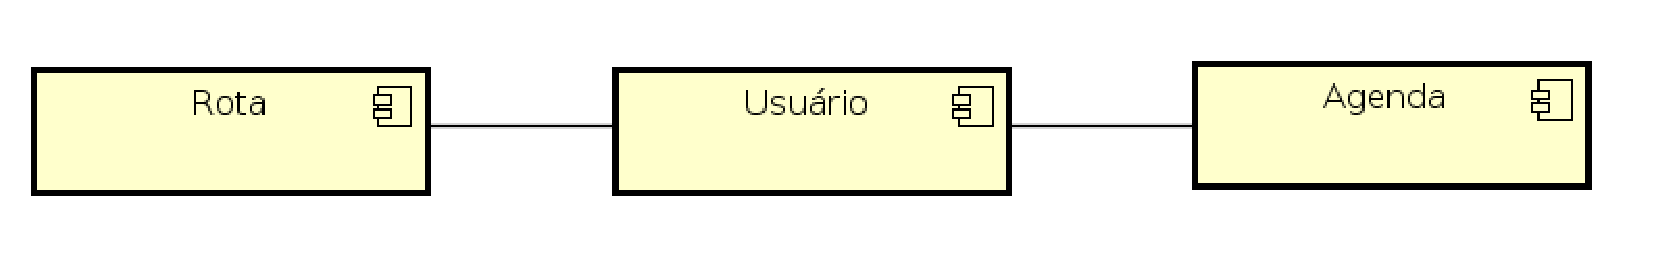
\includegraphics[scale=0.55]{figuras/capitulo5/diagrama_componentes.eps}
	\caption{Diagrama de componentes inicial}
	\label{diagrama de componentes}
\end{figure}

Este modelo servirá como base para a implementação de todas as funcionalidades propostas.

\section{Uso do Framework}

O framework será desenvolvido em \textit{``Ruby on Rails''} e terá sua \textit{``Gem''}\footnote{\url{http://www.akitaonrails.com/2009/2/2/entendendo-rubygems}} publicada em um repositório online para uso de outros desenvolvedores.

Para comprovação do funcionamento do \textit{framework}, este trabalho propõe o desenvolvimento de uma rede social que faça uso do mesmo. Esta rede deverá fazer uso dos principais recursos providos pelo \textit{framework}, dessa forma, pode-se ver o seu uso na prática.

\section{Prova de Conceito}

Foi desenvolvida uma pequena aplicação para implementação de alguns conceitos discutidos neste trabalho.

De modo geral a aplicação desenvolvida implementa uma rede de usuários ligados entre si formando um grafo, conta com as classes Usuário, Aresta que é usada para fazer as ligações entre as entidades e a classe Grafo que representa a própria rede com todos os usuários. Foram implementadas as funcionalidades de relacionamento descritas nas figuras \ref{segue} e \ref{amigo}, além de uma varredura dos usuários presentes no grafo pelos algoritmos de busca ~\nameref{subsec:bfs} e ~\nameref{subsec:dfs}.

Todo o código fonte da aplicação citada pode ser encontrado em \url{https://github.com/TCC-SocialNetwork/concept-test}.

Essa aplicação traz a prova do desenvolvimento do \textit{framework} proposto no ponto de relacionamento de usuários, representa um passo inicial para o desenvolvimento real que se dará na segunda etapa deste trabalho.

\section{Trabalhos Relacionados}

\section{Resumo do Capítulo}
